\chapter{Implementation}

\section{NAO robot}


NAO is a programmable, autonomous, 57 cm tall humanoid robot developed by Aldebaran Robotics, a French startup company. The biped is equipped with several
different sensors, including an inertial measurement unit with accelerometer, gyrometer and four ultrasonic sensors that provide NAO with stability and 
positioning within space, in addition eight force-sensing resistors and two bumpers. It features an Intel ATOM 1,6 GHz CPU, located in the head, that runs
 a Linux kernel and a second CPU located in the torso.


NAO has a total of 25 degrees of freedom (DOF), 11 DOF for the lower part that includes legs and pelvis, and 14 DOF for the upper part that includes trunk, 
arms and head. Each leg has 2 DOF at the ankle, 1 DOF at the knee and 2 DOF at the hip. A special mechanism composed of two coupled joints at each hip equips 
the pelvis. The rotation axis of these two joints are inclined at $45^\circ$ towards the body. This mechanism replaces the classical set of three active rotary joints 
encountered in most humanoid robots.


Aldebaran Robotics provides a complete documentation for the robot, based on a geometric model shown in . The model of the lower body of the robot 
NAO is obtained considering the two legs identical and identically actuated. The two revolute joints that constitute the pelvis and named separately, but 
they essentially represent a unique actuated DOF. To conclude, it is important to remark that, unlike prototypes such as Wabian-2R or LOLA, the foot sole of 
the present version of NAO does not feature any passive or active joint that would enhance higher speed gait performances.


\subsection{NAOqi C++ SDK}
\subsection{CopelliaSim support}


\begin{figure}[h!]
    \centering
    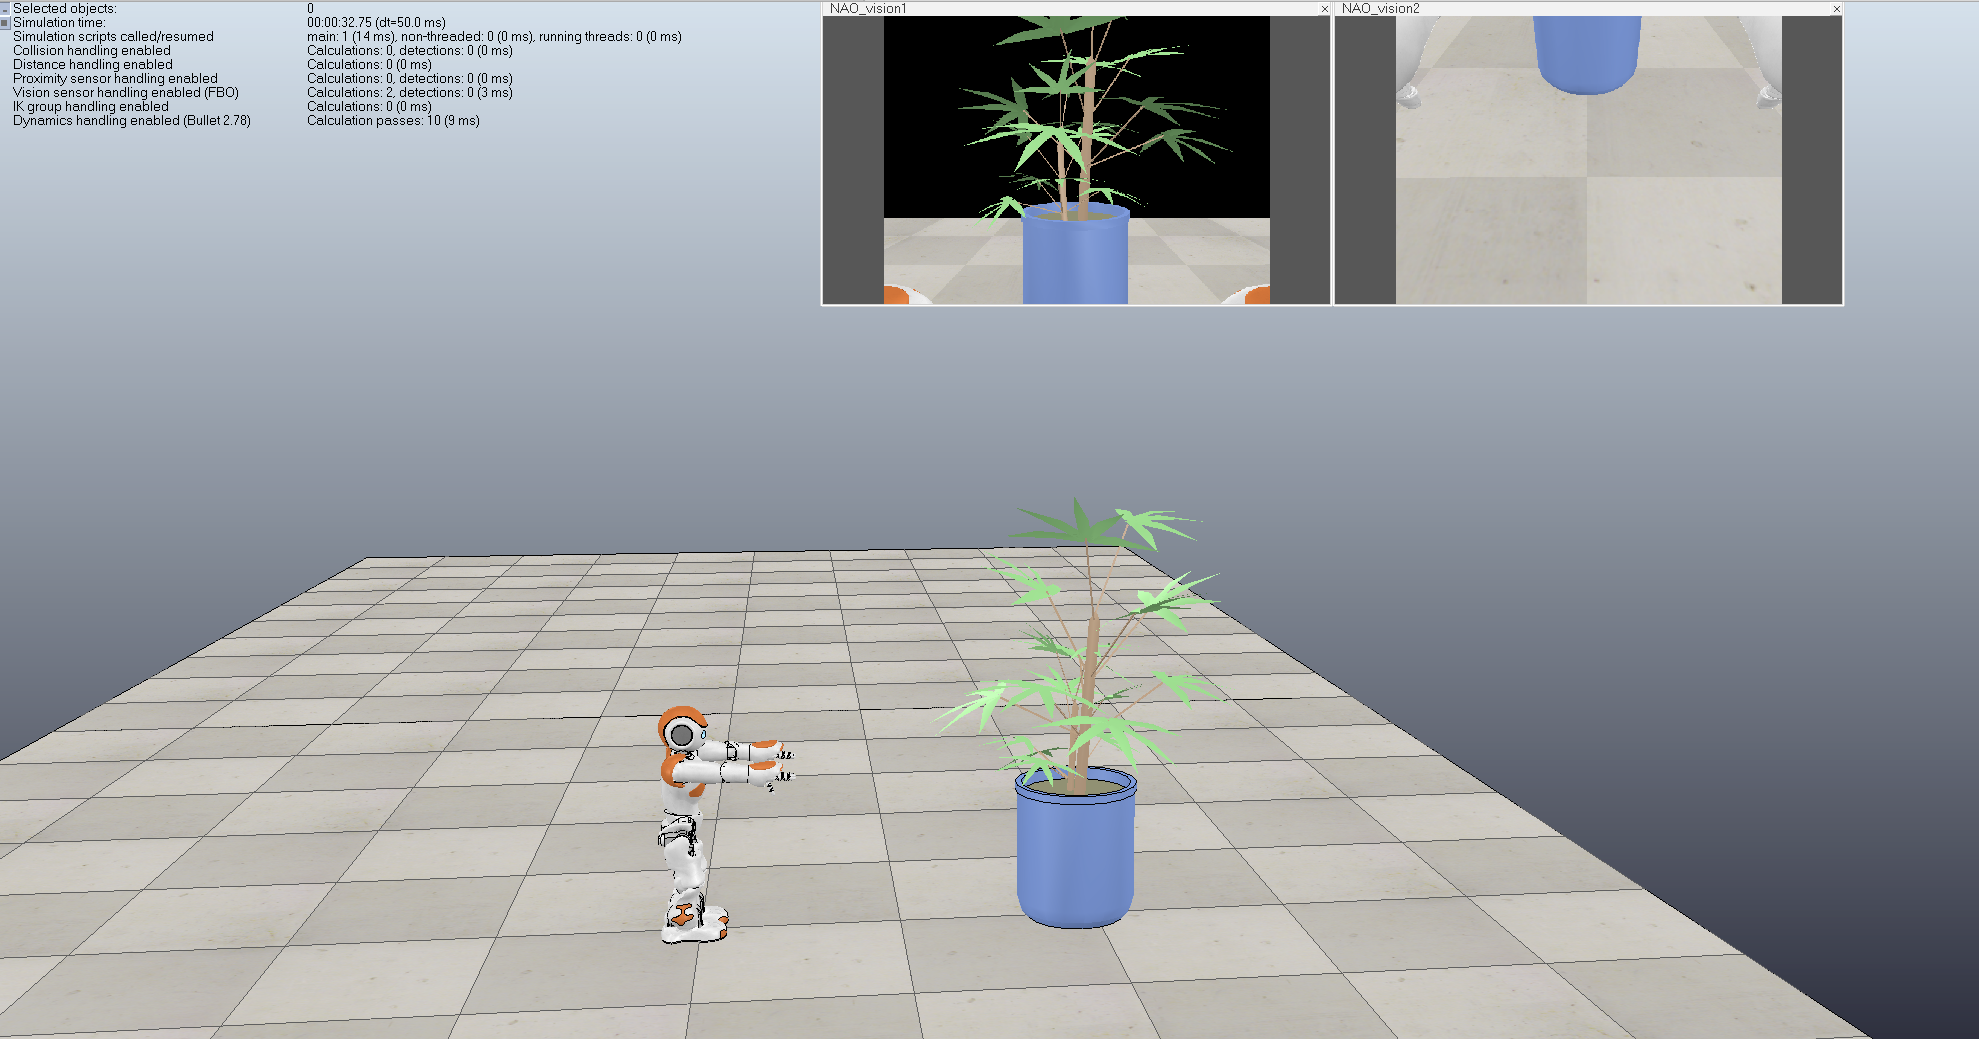
\includegraphics[scale=0.25]{images/copellia-sim.png}\hfill
    \caption{NAO robot in CopelliaSim}\hfill
    \label{fig: copellia-sim}
\end{figure}

\section{Xsens MVN Analyze}
\subsection{Sensor Setup}
\subsection{Xsens Networking Protocol}
\subsection{Network Streaming}
